\chapter{Копырев конец}

Эту главу сложно было втулить. С одной стороны, по местности она подходит сюда идеально, с другой не в тему Логова Змиева, да что поделать?

Через дорогу от холма с Кирилловской церковью лежит урочище Копыловка. Можно сказать что его основа – от перекрестка улиц Телиги и Кирилловской, между Кирилловской и улицей Копыловской, там на углу квартальчик из старых, по четыре-пять этажей, домов. Копыловская 2 построен в 1932, 2-А – 1940, Копыловская 2-Б – 1938, Кирилловская 109/2 – 1927, Кирилловская 109-А – тоже 27-й, дальше на северо-запад идут уже здания построенные позже. А те, что в квартальчике, будто вросли в землю, у некоторых первые этажи подвальные, а к парадным перекинуты мостки. Это потому, что во время Куренёвской трагедии 1961 года уровень грунта поднялся из-за хлынувшей пульпы, нанесло. 

Копыловкой раньше считалась и нынешняя Шполянка, бывшие дачи Шполянского, что теперь лежит по другую сторону от улицы Копыловской. 

Копыловка как бы старое ядро Куренёвки. Старенькая часть района, судя по всему, не застраивалась до упомянутого времени, а на юг от него, вдоль низовья Бабьего яра, по той же стороне, лежало кладбище – на его месте сейчас вход в подземный переход\footnote{50°29'04.9"N 30°28'15.1"E} и на 2023 год сохраняется зеленый пригорок\footnote{50°29'03.6"N 30°28'10.5"E} с подпорной стеной, выше коего стоит дом по адресу Захарьевская, 1. Не знаю, когда эта улица стала Захаровской, но в подлиннике было Захарьевская, еще на плане середины 19 века ее под таким названием видно.

Это кладбище значилось на карте как Общественное, а напротив, на другом берегу Бабьего яра, носившего также имя Вовчего, в роще было кладбище Кирилловских богоугодных заведений.

Я уже кратенько перебрасывал логические мосты от Карпиловки со старых карт и земельных документов к Копыловке. Полагаю сей вопрос решенным, а вот какое название было исконно, Карпиловка ли превратилась в Копыловку, или же Карпиловка слыла одновременно с Копыловкой либо пыталась вытеснить ее, непонятно. 

\begin{center}
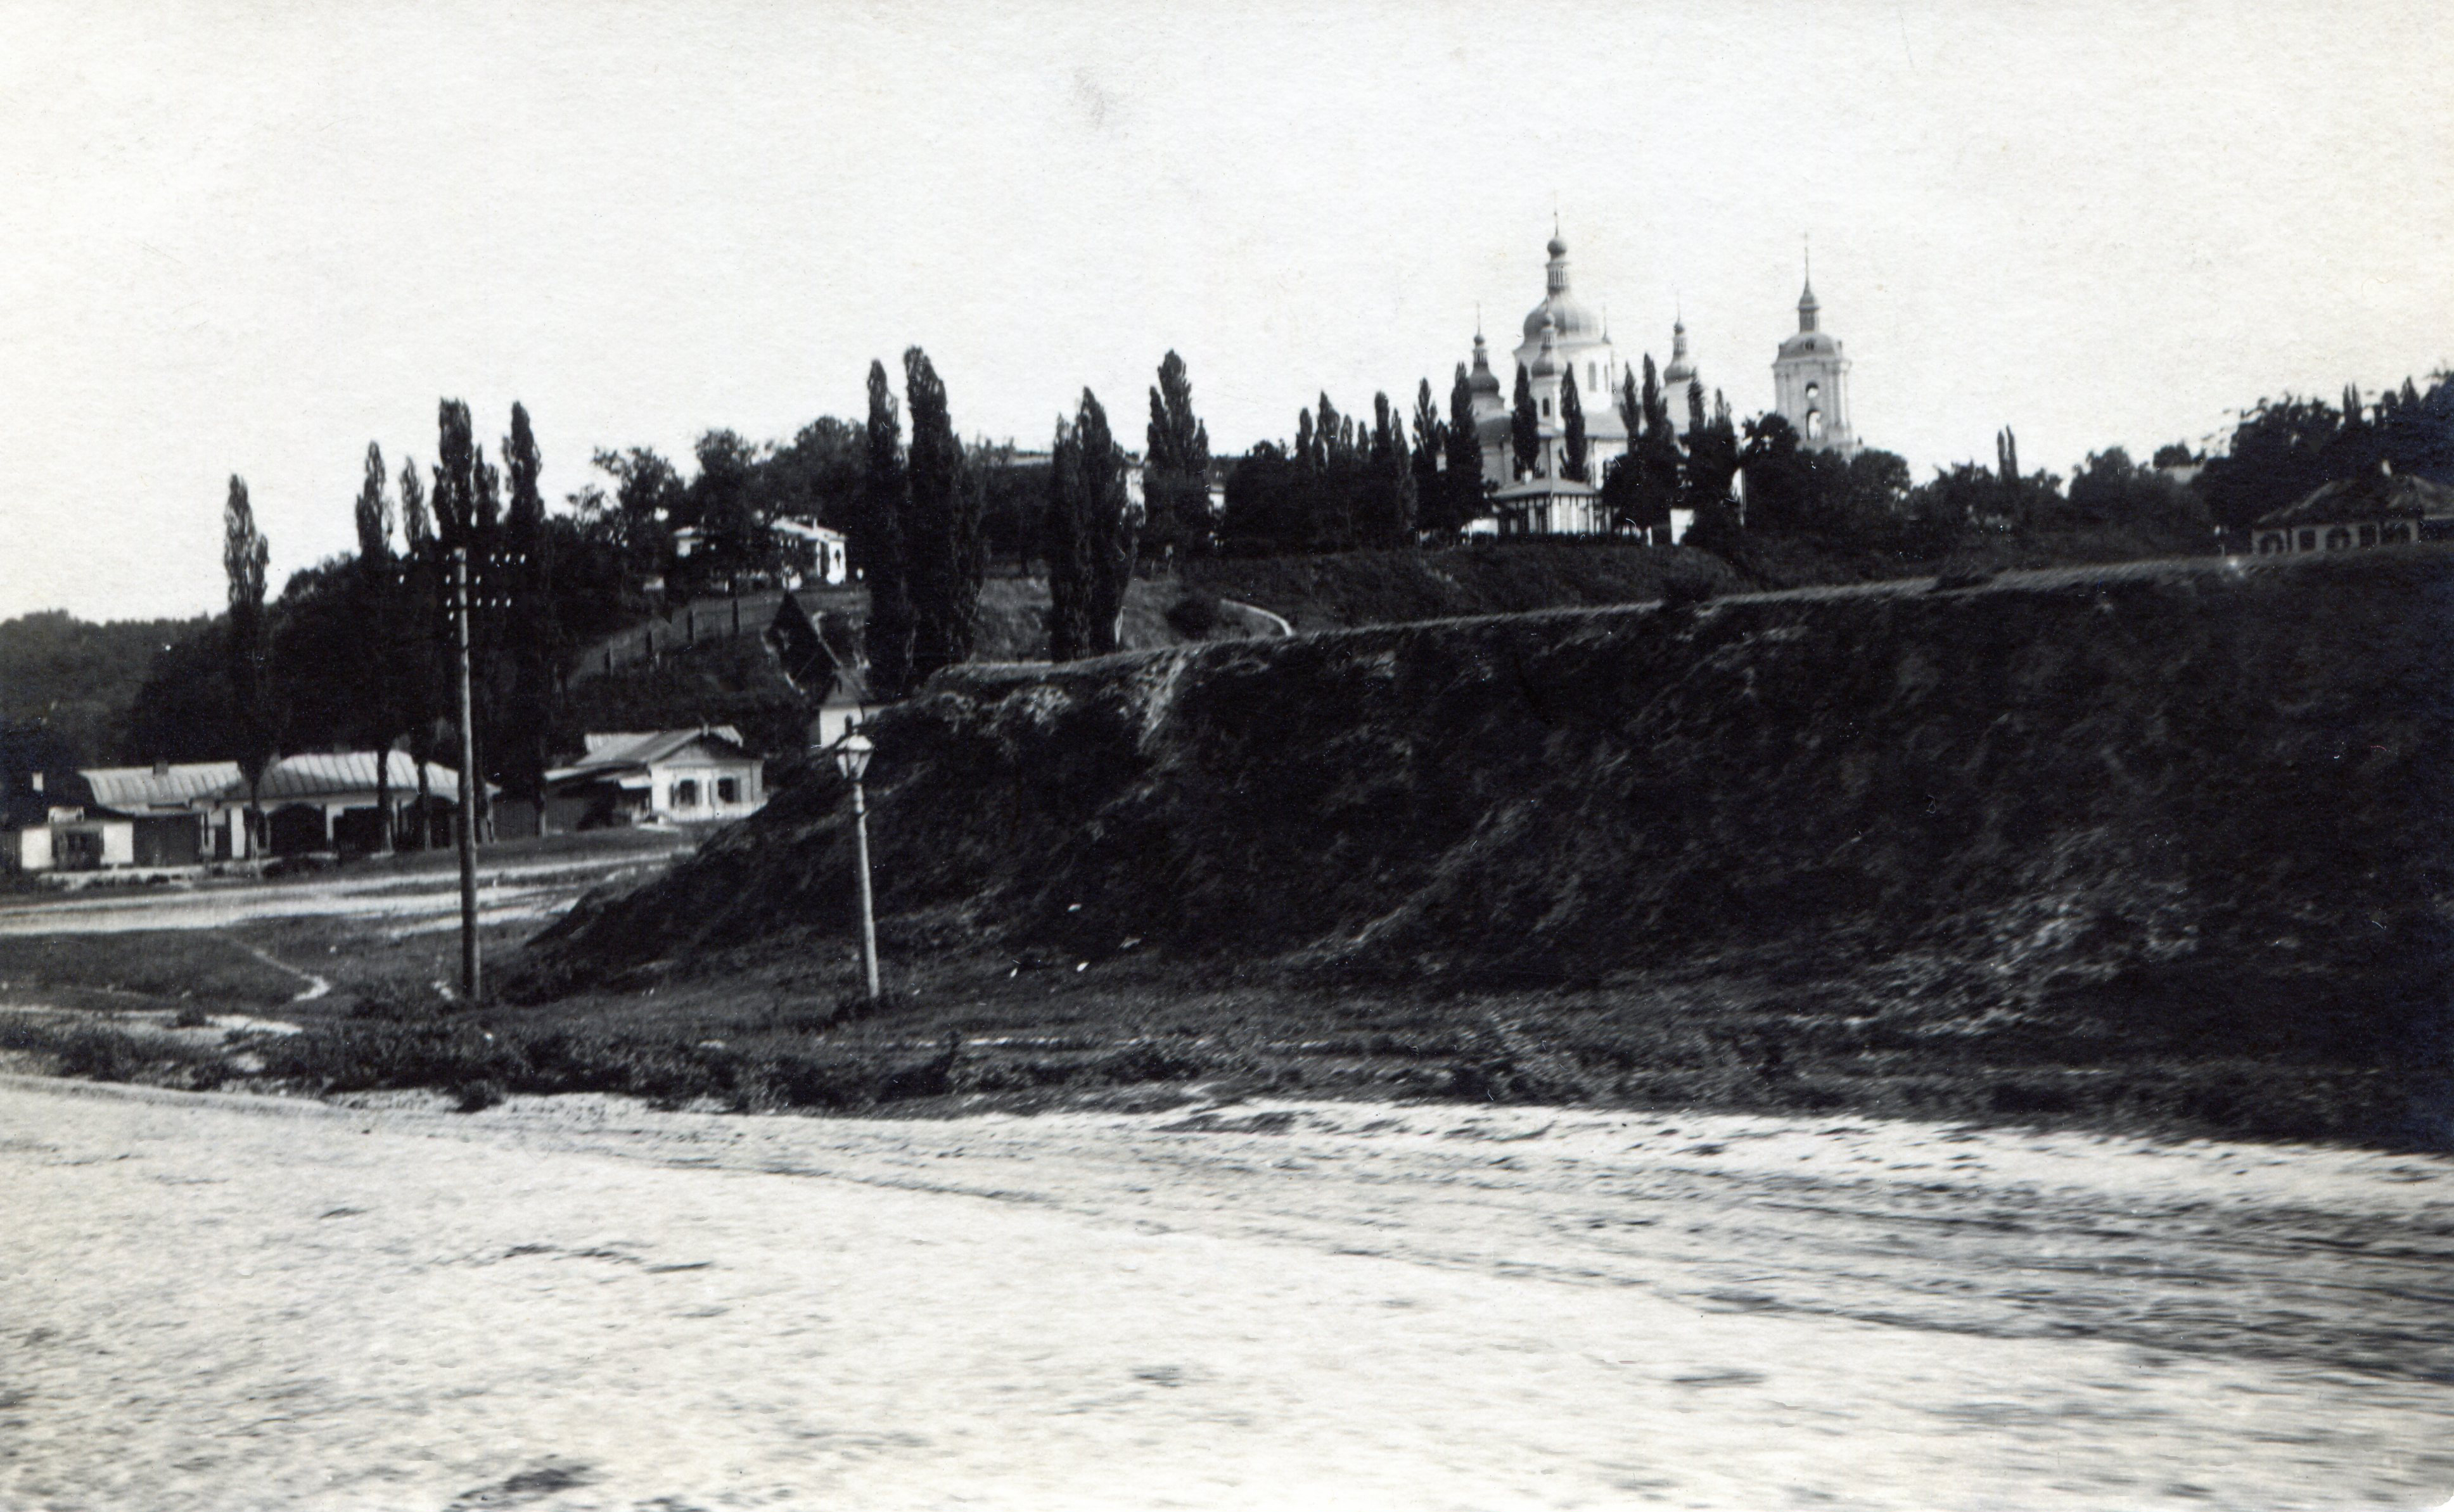
\includegraphics[width=\linewidth]{chast-zmiy/kopyl/mid.jpg}

Стык 19-20 веков, вид через Копыловку (угол справа) на Кирилловскую церковь.
\end{center}

Справедливости ради отмечу, что где-то на Приорке, на 1782 год известен хутор войскового товарища и киевского городового магистрата городского головы Василия Копыстенского, с рощей, прудом и мельницей, но где он находился – я не знаю, да и Карпиловка возникает в документах прежде Копыстенского, посему заключаем, что Копыловка имеет с Карпиловкой общего больше, чем с Копыстенским.

\begin{center}
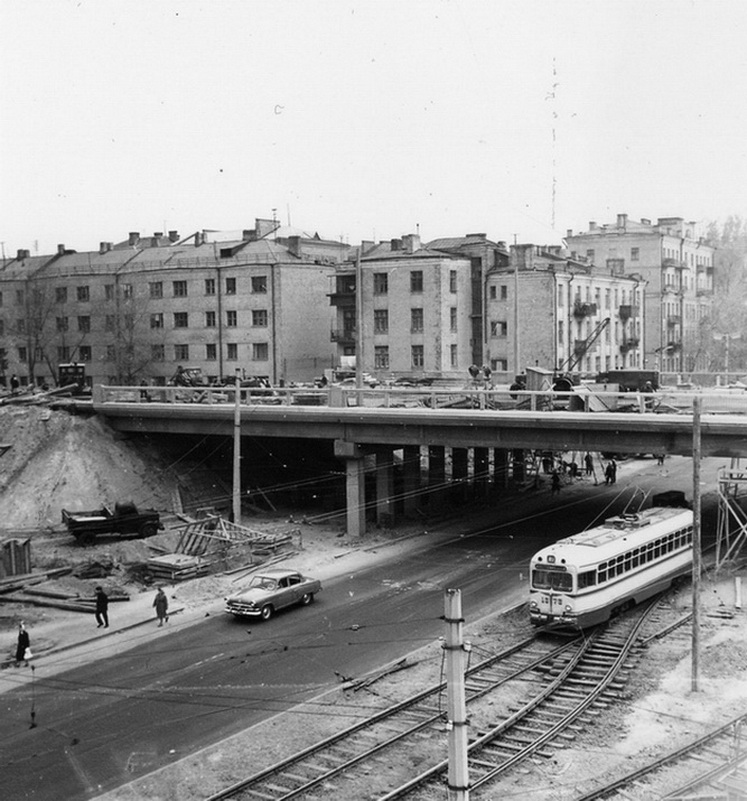
\includegraphics[width=\linewidth]{chast-zmiy/kopyl/1963.jpg}

Вид на угол квартальчика.
\end{center}


Какие же мысли побудили меня отождествить окрестности Копыловки или Карпиловки еще и с летописным Копыревым концом?

Официальная наука полагает оный на горе Воловне, Воловьей, там где Вознесенский спуск. Впрочем, само историческое название – гора Воловня – науке неведомо. Рассуждения о местоположении Копырева конца археологов да историков не лишены логики, впервые их выразил, кажется, еще Петр Лашкарев в работе 1879 года «Развалины церкви св. Симеона и Копырев конец древняго Киева». Рассуждения на то время дельные, но за прошедшее время наука не пыталась их пересмотреть или увязать с б\'ольшим количеством источников.

Что же говорят летописи?

Самое раннее дошедшее до нас, за 1121 год, свидетельство гласит, строками Ипатьевского списка: 

\begin{quotation}
Того же лета заложи святаго Ивана в Копыреве конци.
\end{quotation}

Княжил тогда Владимир Мономах, может он-то и заложил церковь святого Иоанна в Копыреве конци, а может и не он. Позже не сказано, что «свершена бысть», то есть постройка завершена. Просто заложил. А когда свершена, непонятно. Какие урочища рядом – тоже непонятно, связать не с чем. 

Но времена были опасные, а стройматериалы дорогие. Никто построит церковь вне города, условно говоря, в чистом поле. Ее надо возводить внутри пределов крепостной стены, иначе церковь разорят враги. И кто будет ходить в церковь на отшибе? Однако по соображениям официальной науки получается, что вне крепостной стены града Киева, в отдалении, словно сторожевые башни, стояли церкви...

Ипатьевская летопись за 1140 год:

\begin{quotation}
Поиде Всеволод Олгович из Вышегорода к Кыеву, изрядив полкы, и пришед ста у города в Копыреве конци, и начал зажигать дворы, иже суть пред городом в Копыревом конци.\end{quotation}

Делаем вывод, что на пути из Вышегорода, перед городом был некий Копырев конец, а в нем дворы, и вот остановившийся там Всеволод Олгович со своими полками начал эти дворы зажигать.

Получается, между Вышегородом на пути к Киеву ничего стоящего упоминания нет, а перед городом – Копырев конец, и там Всеволод устраивает пожар. Копырев конец представляется мне по этой записи посадом перед городом Киевом, крепостью Киевом.

Ипатьевская, 1147 год, Игорь Олгович убит и свезен на «Подолье на торговище». Прибывает тысяцкий и помещает тело Игоря на ночь в церковь святого Михаила, а потом приезжает игумен, видит нагое тело Игоря, одевает его и 

\begin{quotation}
везе на конец града в манастырь святому 
Семену . бе бо манастырь отца его и деда его Святослава и тамо положиша
\end{quotation}

Отец Игоря – Олег Святославович. Всё верно. Черным по-белому написано также «конец града». Монастырь святого Семена находится на конце града Киева, огороженной части Киева. Отрешитесь от представлений официальной науки, что «град» это пятачок от фуникулера до Софии!

Итак, из написанного делаем вывод, что монастырь святого Семена заложен Святославом Ярославичем (1027-1076), князем черниговским, а с 1073 года киевским. Это был сын Ярослава Мудрого и Ингигерды Шведской. Святослав умер не своей смертью, однако от операции «резания желве», и «положен бысть у Спаса».

Напрямую в летописи не сказано, что Святослав Ярославич заложил во время своей жизни какой-либо монастырь в Киеве, а особено в Копыреве конце. Однако мы знаем, что в 1121 был заложен монастырь святого Ивана в Копыреве конце, и это уже после смерти Святослава Ярославича. Если доверять сведениям летописца, то в Копыреве конце некогда, до 1076 года, Святослав Ярославич заложил святого Семена, а затем некто в 1121 заложил святого Ивана.

Ипатьевская, 1150 год:

\begin{quotation}
В то-же время Святослав Олгович перенесе мощи брата своего Игоря от святаго Семена, ис Копырева конца, в Чернигов 
\end{quotation}

Отсюда мы узнаём, что церковь святого Семена, где лежали мощи Игоря, находится в Копыревом конце. Опять же, монастырь и церковь, служащую княжеской усыпальницей, не будут строить вне города. Мы помним из предыдущей записи, что святого Семена – в конце града, и конец этот, как теперь уточнилось, именуется Копырев.

К тому времени, на 1150 год, историки невесть почему считают, уже построена Кирилловская церковь. Про нее точно известно, что она-то и была была семейной усыпальницей черниговских князей Олговичей. Но если Святослав Олгович переносит мощи брата своего Игоря «от святаго Семена, ис Копырева конца», что нам думать?

Святой Кюрила впервые возникает в Ипатьевской летописи за 1171 год, но об этом позже.

А вот запись, по которой официальная наука и привязала Копырев конец к горе Воловне, памятуя, что святого Ивана заложена в Копыреве конци. Ипатьевский список, 1151:

\begin{quotation}
Вячьслав-же Изяслав и Ростислав повелеша Володимиру пойти с Берендеи и с вежами и с стады их пойти ко Олгове . и сташа мьжи дьбрями от Олговы оли и в огород святаго Іоана а семо оли до Щковицы
\end{quotation}

Дано три ориентира – Олгова, Щековица и огород святого Иоана. Сейчас, как мы знаем, Олегова могила и Щекавица совместились, и как отделить их до исконных значений, неясно. И вот Володимир и Берендеи с вежами и стадами встали меж дебрями от Олговы в огород (огороженное владение) церкви или монастыря святого Иоанна а оттуда до Щековицы.

Если мы нарисуем треугольник между допустим двумя точками на современной Щекавице и одной около Кирилловской церкви, получится, что «огород святого Иоана» это Кирилловские высоты и Татарка. А если повернуть треугольник в другую сторону, на юг, то – ну да, упремся примерно в Кудрявец и Воловню. Исходя из этой последней точки зрения, дебри были в низовьях улицы Глубочицкой, у ее перекрестка с Нижним и Верхним валами, с Вознесенским спуском, Гончарами и Кожемяками. Отличная мишень для стрел с Замковой горы, ну да ладно.

Продолжаем листать летопись далее. Вот любопытное, где нет впрочем прямого упоминания Копырева конца. 

Ипатьеская, за 1161 год гласит, что Изяслав собрался с братьями и послал за Половцами, те пришли к нему. Изяслав с Всеволодичем, Олгом и Половцами поиде за Вышегород к «божници», пробыл там столько-то дней и стал двигаться к Киеву, но как!

Во-первых:

\begin{quotation}
ту же перешедше Днепр у боженки и поиде полки к Киеву и пришедши сташа на болоньи  в лозах противу Дорогожичю
\end{quotation}
  
Не совсем понятно, почему, если Вышегород и Киев на одном берегу, а боженка «за Вышегородом», переходят Днепр у боженки. Боженка была на левом берегу Днепра? 

Далее войско двигается к Киеву и останавливается на болоньи в лозах напротив Дорогожича. Это февраль. Где же болонье? На ум приходит, конечно, если мы спустимся от метро «Дорогожичи» по Бабьему яру, то окажемся как раз в Копыловке. 

Правда, в 18-м веке было известно урочище Поганые Лозы, по карте где-то выше Лукьяновки, может и на Дорогожичах, но у нас есть «болонье», а болонье больше подходит к традиционной Оболони, а значит к низовьям Бабьего Яра. К тому же:

\begin{quotation}
нача Изяслав полкы рядити с братьею и доспев иде к Подолью
\end{quotation}

От Дорогожичей к Подолью как-то неудобно добираться, значит речь идет таки о низменности. Любопытно, почему нападение на Киев готовилось именно от Подола? Так было проще? 

А далее любопытное:

\begin{quotation}
а Ростислав стояше с Андреевичем
подле столпье загорожено бо бяше тогда  столпием от горы оли и до Днепра.\end{quotation}

Ростислав стоял с Андреевичем подле столпья. Столпье загораживало собой тогда (а при летописце уже нет?) от горы и до Днепра. Получается, бревенчатая крепостная ограда. Но от какой горы? Горы в понимании той, что над Подолом – Замковая, а может Щекавица, либо иная возвышенность?

Но столпье... Стоящие бревна, наверное. А слово «копыл» или «копыль», от коего можно вывести Копыловку, означает, по Далю, «стояк,  стоень,  надолба, торцом  вставленная во что деревяшка». Листаем дальше.

Ипатьевская, 1162 год:

\begin{quotation}
Торци же постигоша возы их на Желяни полкы же их постигоша . от Буличь и ту начаша сечи я . а инех руками имати . яша же тогда . и Шварана  и Милятича оба . Степена . и Якуна . и Нажира Переяславича . Изяслава же постигоша к озерам въездяча в борок и постиже и Воибор Генечевичь и сече по главе саблею а другыи  боде и в стегно въдым ѣ . и ту
лете с коня . и взем ѣ Мьстислав ле жива посла в манастырь к святого Семену еже есть  в Копыреве конци
\end{quotation}

Всё что удается отсюда вытянуть про Копырев конец, что в нем был уже монастырь святого Семена, и Мстислав отправил туда еле живого Изяслава, который впрочем скоро умер. Упоминание озер и борка, около которых настигли Изяслава, неясно как относится к расположению святого Семена, но вероятно это был ближайший оттуда монастырь.

Десятилетие спустя в летописях появляется святой Кюрила:

Ипатьевская, 1171:

\begin{quotation}
сняшася братья Вышегороде и пришедше сташа на Дорогожичи . под святым Курилом Феодоровы недели . и второе недели . оступиша вьс град Киев
\end{quotation}

Сравним в тем, как в 1161 году князья останавливались в лозах против Дорогожичей. А сейчас сказано – сташа на Дорогожичи под святым Курилом. Но каждый раз из Вышегорода, там один был путь, по нынешней улице Вышгородской, переходящей в Кирилловскую, примерно.

Судя по всему это было наиболее удобное место для атаки, по крайней мере с севера. Ибо в 980 году князь Владимир, еще не захвативший Киев, а бывший новгородским князем, проделывает то же самое:

Ипатьевский список:

\begin{quotation}
И приде Володимир, к Киеву с вои многыми, и не може Ярополк стати против Володимиру, и затворися Ярополк в Киев с людьми своими и с воеводою Блудом; и стояше Володимир, обрывся на Дорогожичи, межи Дорогожичем и
Капичем, и есть ров и до сего дне.
\end{quotation}

\begin{center}
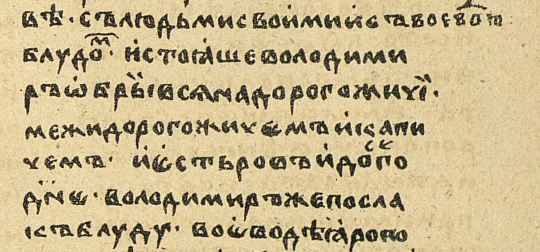
\includegraphics[width=\linewidth]{chast-zmiy/kopyl/kapich.png}
\end{center}

Более чем вероятно, речь идет о той же местности, что потом стала Карпиловкой, Копыловкой, и является, как понимаю, Копыревым концом. Здесь же, за 980 год, Нестор из своего уже времени, спустя несколько веков, называет урочище Капич. Капич, Копырев, Карпиловка, Копыловка, всюду это Кап-Коп-Карп. Нестор жил в 11-12 веках, про Капич он откуда-то переписал, но откуда? И верно ли переписал? А может писец после Нестора?

Капич... Что означает? Капище? Или смысл другой? Капич исказился потом на Копырев?. Ведь кроме версии о сходстве столпья и копыла можно подумать, что Капич – от слова копать. Есть слово «копырсаться» – тоже копать. Копырев не отсюда ли? Вот же,

\begin{quotation}
и стояше Володимир, обрывся на Дорогожичи, межи Дорогожичем и Капичем, и есть ров и до сего дне
\end{quotation}

Володимир там окопался, до времени Нестора сохранился ров. Где же? Название Капич – современное Нестору или же он приводит давний для него топоним? Слишком зыбкая почва для однозначного решения задачи.

Однако мы помним, что Нестор не видел столпие, но писал о нем в прошедшем времени, что тогда-то оно существовало. А ведь где столпие, там должен быть и ров, логично? Быть может, ров не от того, что Володимир обрывся, а потому что ров был при столпие? 

Но вернемся к святому Кюрилу. Ипатьевская летопись, 1178 год:

\begin{quotation}
Того же лета преставися княгини Всеволожая приемьши на ся чернечкоую скимоу положена бысть в Києве у святаго Кюрила юже бе сама создала
\end{quotation}

Лаврентьевский список, за 1202, про князя Романа:

\begin{quotation}
и отвориша ему Кыяне ворота Подольская в Копъıреве конци . и въеха в Подолье . и посла на Гору к Рюрикови . и ко Олговичем . и води Рюрика к кресту
\end{quotation}

Из сего заключаем, что в Копыревом конце были Подольские ворота. Запись купно с показанной мною за 1151 год и есть основания официальной науки считать Копырев конец окрестностями горы Воловни. Но ведь ворота часто именовались по направлению, куда они ведут. Ворота Ерданские с плана Ушакова не окол Иорданского монастыря, но от них начинается дорогоа в его сторону. Ворота Крещатицкие, сходным образом, на пути к урочищу Крещатик. 

Зацепок, что Копырев конец это Капич, Карпиловка и Копыловка гораздо больше. И разнобой в именовании тамошней церкви меня не смущает, а напротив убеждает в верности своего вывода, ибо Олговичи хоронили своих в «отней» церкви, а таковой считают Кирилловскую, но вот Игоря Олговича положили сначала в святого Семена! Да поясняется:

\begin{quotation}
бе бо манастырь отца его и деда его Святослава и тамо положиша
\end{quotation}

Тоже монастырь отень! Не это ли указание на одно и то же место, но под разными именами?

Если мы составим список по годам, то получаются следующие упоминания церквей-монастырей, как предполагаю, на одном месте:

\medskip

1121 – Ивана

1150 – Семена

1151 – Иоана

1162 – Семена

1171 – Курила

1178 – Кюрила

\medskip

Семен, или, как его сейчас называют, Симеон... Адриан Прахов в небольшой статье «Открытие фресок Кирилловского монастыря под Киевом» 1883 года сообщает, кроме прочего:

\begin{quotation}
Интересная находка ждала нас на столпах царской арки, закрытых иконостасом. По снятии иконостаса и по очистке эти столпы оказались сверху и до низ покрытыми фресками. На северном их них изображена Богоматерь с Предвечным младенцем на руках, за нею слева пр. Иосиф с парою голубков. На соответствующих местах южного столпа изображены св. Богоприимец Симеон и св. Пророчица Анна.
\end{quotation}

Впрочем, главной находкой были 12 бытовых картин из жития Кирилла Александрийского, святого Кюрилы. Несомненно, что и в древности эта церковь была посвящена ему, однако не могла ли она прежде создания фресок быть посвящена другому святому, или же рядом находился какой-то другой храм, а хоть бы деревянный, или же деревянный был на месте Кюрилы? Над той пещерой, о которой я рассказывал. Или в ней самой. Пещерный храм.

Что, ежели не случайно более популярный Симеон – Столпник, и в летописи упомянуто «столпие»?

Известна икона в разных вариантах, где изображены сразу трое – Симеон Столпник, Иоанн Богослов и апостол Филип. Одной из традиций изображения Иоанна Богослова было рисовать его на фоне пещеры, ибо Иоанн перед тем, как диктовать священный текст своему ученику Прохору, на 10 дней затворился в пещере. Что же, пещера есть, точно под церковью святого Кюрилы.

Попытаюсь восстановить хронику и развеять путаницу.

Дано – горка с нынешней Кирилловской церковью.

Князь Святослав Ярославич (1027-1076), сын Ярослава Мудрого, в крещении Николай, заложил монастырь Семена, опёка коего продолжилась сыном его Олегом. Про обоих сказано, применительно к Игорю Олговичу:

\begin{quotation}
везе на конець града в манастырь святому 
Семену . бе бо манастырь отца его и деда его Святослава и тамо положиша
\end{quotation}

Затем, в 1178 году умирает княгиня Всеволожая: 

\begin{quotation}
Того же лета преставися княгини Всеволожая приемьши на ся чернечкоую скимоу положена бысть в Киеве у святаго Кюрила юже бе сама создала
\end{quotation}

Юже бе сама создала – то есть монастырь именно Кюрила создала княгиня Всеволожая, а не Всеволод, как часто пишут историки. Полагаю, создала на месте прежнего Семенова монастыря. По хронике мы видим, что как только исчезает упоминание Семенова, появляется Кюрила. И оба несут функцию родовых монастырей и усыпальниц Олговичей. Очевидно, монастырь Семена продолжился Кюрилом.

А что за княгиня Всеволожая? Поскольку умерла она в 1178, а до этого святой Курило упомянут в 1171 году, именно эта Всеволожая княгиня построила святого Курилу по крайней мере к 1171 году, а в 1178 умерла.

В том же 1178 году Всеволод Святославич по прозвищу Чермный женился на жене «из Ляхов», дочери Казимира, во Филипово говенье. Согласно общепринятому мнению, это была дочь по имени Мария. Но ведь не она та «княгиня Всеволожая», что прежде, к 1171 построила святого Курила.

Всеволожей летописец мог назвать, например, жену Всеволода Олговича (сына Олга Святославича), который родился вероятно в 1094 и умер 1 августа 1146. Эта княгиня Всеволожая (имя в Повести временных лет не указано) была, по сопоставлениям сведений из летописи, дочерью Киевского князя Мстислава Владимировича и шведской принцессы Христины, родилась в 1110 или 1113 году. Возможно именно она была погребена в святом Куриле.

Почему же Курило? У Всеволода Олговича либо христианское имя было Кирилл, во всяком случае, таково общепринятое мнение, и существуют свинцовые вислые печати, связываемые со Всеволодом Олговичем, и на них написано «господи помози рабу своему курилу».

А как же быть со святым Иоаном? Предположу, что Иван и был начальным посвящением монастыря на том же месте. «Ивана», как мы помним, в 1121 году заложили при княженьи Владимире Мономаха.

Хорошо, есть ли какие-то более поздние данные насчет Копырева конца или чего-либо Копырева вообще? Как ни странно, есть – уже и много позже Карпиловки. Но, чем считалась Карпиловка?

Напомню разграничение земель на 1701 год:

\begin{quotation}
Аби люде, на подворках Карпиловкою прозываемых, близко места Киева, от монастыра паненского Иорданского и от монастыра Кирилского мешкаючи, по самый поток, межи горами Шкавицей и Лисою будучи, належали непременно до монастыра Кирилскаго
\end{quotation}

То бишь Карпиловка это пространство между Кирилловским монастырем и потоком, что протекал по нынешней улице Нижнеюрковской. Одним словом, местность, слывущая Кирилловскими высотами.

А поглядим на кусок карты 1860 года, где изображены этим самые высоты.

\begin{center}
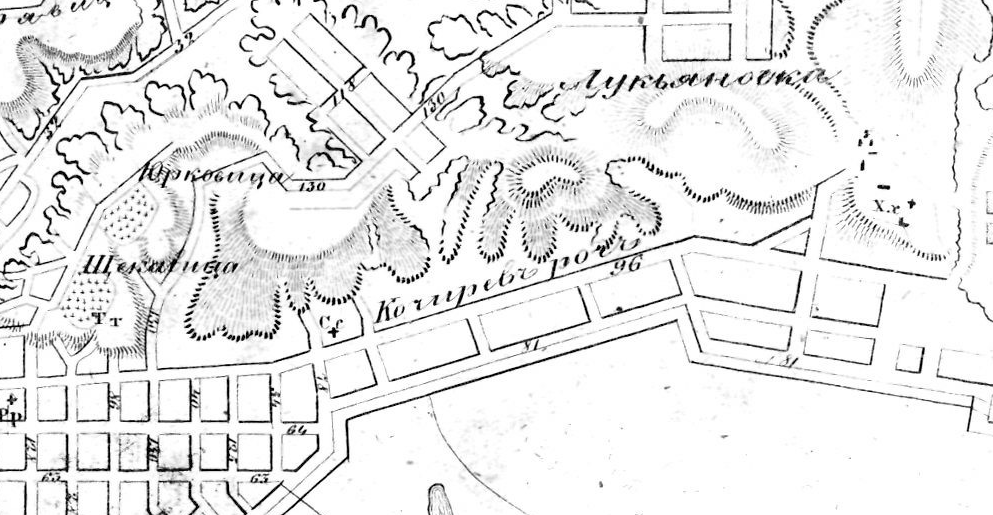
\includegraphics[width=\linewidth]{chast-zmiy/kopyl/1860.png}
\end{center}

Я кадрировал карту таким образом, чтобы важная для нас надпись была примерно посередине. Как это читать? «Копиревъ рогъ»? 

\begin{quotation}
Поиде Всеволод Олгович из Вышегорода к Кыеву, изрядив полкы, и пришед ста у города в Копыревом конци, и начал зажигать дворы, иже суть пред городом в Копыревом конци.\end{quotation}

Если двигаться по улице Вышгородской к Кирилловской, мы прибудем точно в урочище Копылово.... 

Однако нам тут делать больше нечего, отправимся южнее, вернемся на Смородинский спуск, но сначала разберем еще один вопрос.